\begin{enumerate}
\item In \figref{fig:circ.jpg}, from an external point $P$,two tangents $PQ$ and $PR$ are drawn to a circle of radius $4cm$ with centre $O$. If $\angle QPR=90\degree$ ,then length of $PQ$ is 
\begin{enumerate}[label=(\Alph*)]
\item $3cm$
\item $4cm$
\item $2cm$
\item $2\sqrt{2}cm$
\begin{figure}[H]
\centering
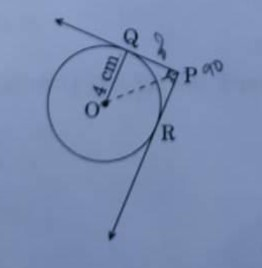
\includegraphics[width=\columnwidth]{figs/circ.jpg}
\caption{}
\label{fig:circ.jpg}
\end{figure}
\end{enumerate}
\item In \figref{fig:circ2.jpg}, $PQ$ is tangent to the circle with centre at $O$, at the point $B$. If $\angle AOB=100\degree$, then $\angle ABP$ is equal to
\begin{enumerate}[label=(\Alph*)]
\item $50\degree$
\item $40\degree$
\item $60\degree$
\item $80\degree$
\begin{figure}[H]
\centering                                       
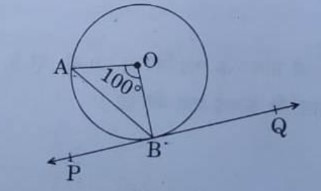
\includegraphics[width=\columnwidth]{figs/circ2.jpg}  
\caption{}
\label{fig:circ2.jpg}                      
\end{figure}
\end{enumerate}
\item In \figref{fig:circ3.jpg}, a quardilateral $ABCD$ is drawn to circumscribe a circle.\newline Prove that \newline $AB+CD=BC+AD$.
\begin{figure}[H]
\centering
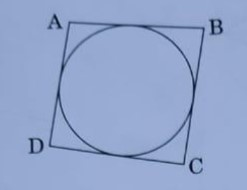
\includegraphics[width=\columnwidth]{figs/circ3.jpg}
\caption{}
\label{fig:circ3.pjpg}
\end{figure}
\item In \figref{fig:circ4.jpg}, find the perimeter of$\triangle{ABC}$, if $AP=12$cm.
\begin{figure}[H]
\centering
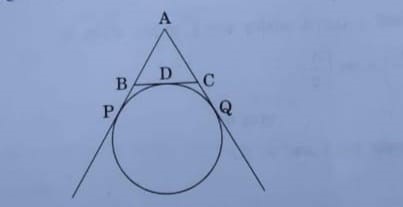
\includegraphics[width=\columnwidth]{figs/circ4.jpg}
\caption{}
\label{fig:circ4.jpg}
\end{figure}
\end{enumerate}